\documentclass[oneside,12pt,english]{book}
\usepackage{babel}
\usepackage[utf8]{inputenc}
\usepackage{color}
\definecolor{marron}{RGB}{60,30,10}
\definecolor{darkblue}{RGB}{0,0,80}
\definecolor{lightblue}{RGB}{80,80,80}
\definecolor{darkgreen}{RGB}{0,80,0}
\definecolor{darkgray}{RGB}{0,80,0}
\definecolor{darkred}{RGB}{80,0,0}
\definecolor{shadecolor}{rgb}{0.97,0.97,0.97}
\usepackage{graphicx}
\graphicspath{{img/}{01-this-is-fairys-album/img/}}
\usepackage{wallpaper}
\usepackage{wrapfig,booktabs}

\usepackage{fancyhdr}
\usepackage{lettrine}
\input Acorn.fd
\newcommand*\initfamily{\usefont{U}{Acorn}{xl}{n}}

\usepackage{geometry}
\geometry{
tmargin=5cm, 
bmargin=5.2cm, 
lmargin=5cm, 
rmargin=3cm,
headheight=1.5cm,
headsep=0.8cm,
footskip=0.5cm}


% \usepackage[full]{textcomp}
\renewcommand{\familydefault}{pplj} 
\usepackage[
final,
stretch=10,
protrusion=true,
tracking=true,
spacing=on,
kerning=on,
expansion=true]{microtype}

\setlength{\parskip}{1.3ex plus 0.2ex minus 0.2ex}


\usepackage{fourier-orns}

\newcommand{\ornamento}{\vspace{2em}\noindent \textcolor{darkgreen}{\hrulefill~ \raisebox{-2.5pt}[10pt][10pt]{\leafright \decofourleft \decothreeleft  \aldineright \decotwo \floweroneleft \decoone   \floweroneright \decotwo \aldineleft\decothreeright \decofourright \leafleft} ~  \hrulefill \\ \vspace{2em}}}
\newcommand{\ornpar}{\noindent \textcolor{darkgreen}{ \raisebox{-1.9pt}[10pt][10pt]{\leafright} \hrulefill \raisebox{-1.9pt}[10pt][10pt]{\leafright \decofourleft \decothreeleft  \aldineright \decotwo \floweroneleft \decoone}}}
\newcommand{\ornimpar}{\textcolor{darkgreen}{\raisebox{-1.9pt}[10pt][10pt]{\decoone \floweroneright \decotwo \aldineleft \decothreeright \decofourright \leafleft} \hrulefill \raisebox{-1.9pt}[10pt][10pt]{\leafleft}}}

\makeatletter
\def\headrule{{\color{darkgreen}\raisebox{-2.1pt}[10pt][10pt]{\leafright} \hrulefill \raisebox{-2.1pt}[10pt][10pt]{~~~\decofourleft \decotwo\decofourright~~~} \hrulefill \raisebox{-2.1pt}[10pt][10pt]{ \leafleft}}}
\makeatother

\fancyhf{}

\renewcommand{\chaptermark}[1]{\markboth{#1}{}}
\renewcommand{\sectionmark}[1]{\markright{#1}}

\newcommand{\estcab}[1]{\itshape\textcolor{marron}{\nouppercase #1}}

\fancyhead[LE]{\estcab{ESL in Action}}
\fancyhead[RE]{\estcab{This is Fairy's Album}}
% \fancyhead[CE,CO]{\estcab{\decoone}}
%\fancyhead[LO]{\estcab{\rightmark}} % malo cuando no hay section ~~~ \thesection
%\fancyhead[RO]{\estcab{\leftmark}}
\fancyhead[LO]{\estcab{This is Fairy's Album}} % malo cuando no hay section ~~~ \thesection
\fancyhead[RO]{\estcab{ESL in Action}}

% \fancyhead[RO]{\bf\nouppercase{ \leftmark}}
% \fancyfoot[LE]{\bf \thepage ~~ \leafNE}
% \fancyfoot[RO]{ \leafNE  ~~ \bf \thepage}

\fancyfoot[LO]{
  \ornimpar \\ \small \sffamily \textcolor{darkgray}{\emph{Live After 60}} 
  \hfill \bf \textcolor{darkgreen}{\leafNE} ~~~ \textcolor{darkgray}{\thepage}}

\fancyfoot[RE]{
  \ornpar \\ \small \sffamily \textcolor{darkgray}{\textbf{\thepage ~~~
  \reflectbox{\textcolor{darkgreen}{\leafNE}}}}  \hfill 
  \textcolor{darkgray}{\emph{Live After 60}}}

\newenvironment{Section}[1]
{\section{\vspace{0ex}#1}}
{\vspace{12pt}\centering ------- \decofourleft\decofourright ------- \par}



\usepackage{lipsum}
\setlength{\parindent}{1em} % Sangría española
\pagestyle{fancy}

\renewcommand{\footnoterule}{\vspace{-0.5em}\noindent\textcolor{marron}{\decosix \raisebox{2.9pt}{\line(1,0){100}} \lefthand} \vspace{.5em} }
\usepackage[hang,splitrule]{footmisc}
\addtolength{\footskip}{0.5cm}
\setlength{\footnotemargin}{0.3cm}
\setlength{\footnotesep}{0.4cm} 

\usepackage{chngcntr}
\counterwithout{figure}{chapter}
\counterwithout{table}{chapter}

\usepackage{caption}
\usepackage{tikzsymbols}
\usepackage{float}
\usepackage{pdfpages}


\begin{document}

\begin{titlepage}
  \includepdf[pages=1-2,pagecommand={}]{cover.pdf}
  \thispagestyle{empty}
\end{titlepage}

 \TileWallPaper{614pt}{800pt}{scroll.jpg}

\newpage
\setcounter{page}{3}

\section*{This is Fairy's Album.}

\Large
\lettrine[lines=3]{\initfamily\textcolor{darkgreen}{T}}{his} is Fairy, bright as
Spring,\\
Loving every living thing\\
With a love so sweet and true,\\
That all creatures love her too!\\
This is Fairy, bright as Spring,\\
\textsc{In Fairy's Album}.

\begin{figure}
\centering
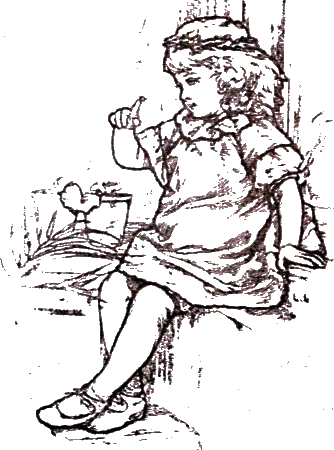
\includegraphics[height=2.8in]{fig01.png}
\end{figure}

This is Fairy, wondrous wise,\\
Sunshine laughing in her eyes,\\
Who will prattle on for hours\\
To the brooks and trees and flowers,\\
To the birds and butterflies,\\
To all creatures `neath the skies,\\
Understanding all they say\\
In a curious sort of way!\\
This is Fairy, wondrous wise,\\
\textsc{In Fairy's Album}.

\begin{figure}
\centering
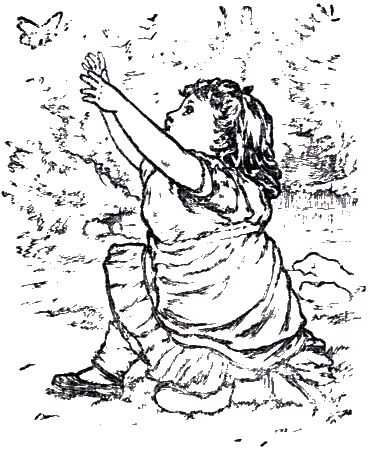
\includegraphics[height=2.8in]{fig02}
\end{figure}

This is Fairy Fanciful,\\
Never moping, never dull,\\
For her mind is amply stored\\
With an overflowing hoard\\
Of the tales of fairy times,\\
And of quaint old nursery rhymes,\\
So that she can always find\\
Good companions when inclined!\\
This is Fairy Fanciful,\\
\textsc{In Fairy's Album}.

\ornamento

\end{document}
